% Complete documentation on the extended LaTeX markup used for Python
% documentation is available in ``Documenting Python'', which is part
% of the standard documentation for Python.  It may be found online
% at:
%
%     http://www.python.org/doc/current/doc/doc.html

\documentclass{manual}

\title{Gheat}

\author{Chad W. L. Whitacre}

\usepackage{graphicx}

% Please at least include a long-lived email address;
% the rest is at your discretion.
\authoraddress{
	Zeta Design \&\ Development \\
	\url{http://www.zetadev.com/software/gheat/} \\
	Email: \email{\ulink{chad@zetaweb.com}{mailto:chad@zetaweb.com}}
}

\date{April 29, 2008} % update before release!
%\date\today
				% Use an explicit date so that reformatting
				% doesn't cause a new date to be used.  Setting
				% the date to \today can be used during draft
				% stages to make it easier to handle versions.

\release{0.2}   % release version; this is used to define the
				        % \version macro

\begin{document}

\maketitle

\begin{abstract}

\noindent

Gheat is a heatmap tile server for Google Maps. Gheat solves the problem of
presenting data on a Google map when there is too much data to be
well-visualized by map markers.

\end{abstract}


\chapter{Introduction}
\label{introduction}

\ulink{Google Maps}{http://maps.google.com/} provides \ulink{a JavaScript
API}{http://code.google.com/apis/maps/} for integrating their maps with your
website. The API includes calls to add markers on the map for various data
points, but this only works when the number of markers placed on any given map
view is relatively small. Gheat solves the problem of presenting data on a
Google map when there is too much data to be well-visualized by map markers. It
does so by using another of the JavaScript API's Google makes available,
whereby additional tilesets can be layered on top of the base map tileset.
(Google Maps works by splitting map imagery into 256x256 pixel tiles and then
knitting them together client-side.)

Gheat runs as a standalone web application under the Aspen webserver. Data 
points are stored in a SQLite database, with each data point uniquely identified
and timestamped. You modify the data in this database using a bundled script, 
run from the command line. The script reads data you provide in a CSV file and 
updates the database accordingly.

Gheat only generates tiles containing data when requested, and it stores these
tiles on the filesystem for future use. On subsequent requests, if no data
relevant to the tile has changed, then the image is served straight from the
filesystem. This saves considerable processing time. Most tiles will be empty,
however, and Gheat precreates empty tiles for all zoom levels and serves the
same file for all empty tiles at a given zoom level. This saves considerable
disk space. These tile caches are organized on the filesystem under the name of
each color scheme in the root of the gheat distribution. Under each such
directory, there is a directory for each zoom level (named \file{0}, \file{1},
\file{2}, etc.), and another called \file{empties}. Gheat will create and
recreate tile cache directories as necessary, and tile caches can be safely
deleted at any time.

Because of the cost of generating heatmaps, Gheat is probably not suitable for
realtime applications. But Gheat performs well when the underlying dataset
evolves on a weekly or even daily basis.


\chapter{Installation}
\label{installation}

\section{The Short Version}

\begin{itemize}
\item{Install \ulink{Python}{http://www.python.org/} (version 2.5 or newer).}
\item{Install \ulink{Aspen}{http://www.zetadev.com/software/aspen/} (version 0.8 or newer).}
\item{Download the Gheat distribution.}
\item{Install \ulink{Pygame}{http://www.pygame.org/} or \ulink{PIL}{http://www.pythonware.com/products/pil/}.}
\item{Start \program{aspen} in the Gheat distribution.}
\item{Add a \ulink{GTileLayerOverlay}{http://code.google.com/apis/maps/documentation/reference.html#GTileLayerOverlay} to your embedded Google Map.}
\end{itemize}


\section{The Long Version}

Gheat involves setting up a web application server, and then wiring up your
web pages to make calls to that server via Google's JavaScript Maps API.

The server side of Gheat has a few dependencies. The first is
\ulink{Python}{http://www.python.org/}. You need version 2.5 or newer, because
Gheat requires the SQLite library, which was added to the standard library in
2.5. There is also some 2.5 syntax in Gheat.  The second is
\ulink{Aspen}{http://www.zetadev.com/software/aspen/}, which is a Python
webserver. Gheat is known to work with Aspen version 0.8. At this point you can
download and unpack the Gheat distribution, or check it out or export it from
the Subversion repository. The next dependency is an imaging library; Gheat
supports both \ulink{Pygame}{http://www.pygame.org/} and
\ulink{PIL}{http://www.pythonware.com/products/pil/} (if you install Pygame,
you only need the imaging components). You can either install it locally in the
\file{__} directory of the Gheat distribution (the
\ulink{virtualenv}{http://pypi.python.org/pypi/virtualenv} tool is a great way
to manage this directory), or you can install it globally. The pygame backend
is three or four times faster than PIL, but PIL is easier to install.  The
functionality is the same with both.

Once all dependencies are satisfied, run the \program{aspen} program within the
Gheat distribution, which is an Aspen website root. The Gheat distribution
includes a sample database out of the box, so at this point you should be able
to hit the webserver now running on your machine and see a heatmap tile. Try
this URL:
\ulink{http://localhost:8080/classic/4/4,6.png}{http://localhost:8080/classic/4/4,6.png}.

\begin{figure}[htp]
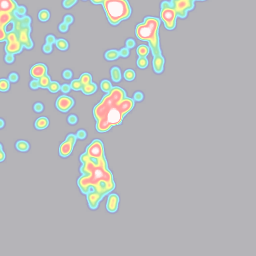
\includegraphics[bb=0 0 256 256]{img/4,6.png}
\caption{A heatmap tile}\label{fig:tile}
\end{figure}

If you see an image like in Figure 2.1, then congratulations! You have
successfully installed the Gheat server.

Once you get the server running, you need to set things up on the client side.
First, you need to embed a \ulink{Google
Map}{http://code.google.com/apis/maps/} on a web page. Then you need to define
a new map layer using
\ulink{GTileLayer}{http://code.google.com/apis/maps/documentation/reference.html#GTileLayer}
and
\ulink{GTileLayerOverlay}{http://code.google.com/apis/maps/documentation/reference.html#GTileLayerOverlay}.
There is an example at \file{example.html} in the Gheat distribution to get you
started. With your Gheat server running, hit
\ulink{http://localhost:8080/example.html}{http://localhost:8080/example.html}
to see it in action (you may need to tweak the Google Maps API key). If it
works, you will see the heatmap tiles loaded overtop of the underlying Google
Map, and you will feel pumped.

\begin{seealso}
\seelink{http://www.zetadev.com/software/aspen/}{Aspen}{The homepage for the Aspen webserver}
\seelink{http://code.google.com/apis/maps/}{Google Maps}{The homepage for the Google Maps API}
\seelink{http://www.pythonware.com/products/pil/}{PIL}{The homepage for the Python Imaging Library (PIL)}
\seelink{http://www.pygame.org/}{Pygame}{The homepage for the Pygame library}
\seelink{http://www.python.org/}{Python}{The homepage for the Python programming language}
\seelink{http://pypi.python.org/pypi/virtualenv}{virtualenv}{The homepage for virtualenv, a tool to create isolated Python environments}
\end{seealso}



\chapter{Configuration}
\label{configuration}

Gheat responds to three configuration options. These are located in the
INI-formatted file \file{__/etc/aspen.conf}, under a section named
\code{[gheat]}. The three options are:

\begin{tableiii}{l|l|l}{var}{Option}{Description}{Defaults}
\lineiii{backend}{The backend library to use for image generation; either 
\code{Pygame} or \code{PIL} (case-insensitive). \code{Pygame} is three or four 
times faster than \code{PIL}, but \code{PIL} can be easier to 
install}{\code{Pygame} if available, then \code{PIL}}
\lineiii{zoom_opaque}{The zoom level at and below which the master opacity will 
be 100\%}{-3}
\lineiii{zoom_transparent}{The zoom level at and above which the master opacity 
will be 0\%}{15}
\end{tableiii}

Here is an example \file{aspen.conf} file:

\begin{verbatim}
[gheat]
backend=PIL
zoom_opaque=-1
zoom_transparent=11
\end{verbatim}


\section{Master Opacity}

Google Maps' zoom level is zero-indexed, starting furthest out. As of this
writing there are 20 zoom levels in use, so the highest available zoom level
(closest in) is 19. The master opacity for Gheat will be scaled linearly between
\var{zoom_opaque} and \var{zoom_transparent}. So, for example, with the default
settings (-3 to 15), the master opacities for each available zoom level are as 
follows.

\begin{tableii}{l|l}{}{Zoom}{Opacity}
\lineii{0}{82.8\%}
\lineii{1}{77.3}
\lineii{2}{71.9} 
\lineii{3}{66.4} 
\lineii{4}{60.5}
\lineii{5}{55.1}
\lineii{6}{49.6}
\lineii{7}{44.1}
\lineii{8}{38.7}
\lineii{9}{33.2}
\lineii{10}{27.3}
\lineii{11}{21.9}
\lineii{12}{16.4}
\lineii{13}{10.9}
\lineii{14}{5.5}
\lineii{15}{0.0}
\lineii{16}{0.0}
\lineii{17}{0.0}
\lineii{18}{0.0}
\lineii{19}{0.0}
\end{tableii}


If \var{zoom_transparent} is less than or equal to \var{zoom_opaque}, the
opacity will be 100\% for all zoom levels. The master opacity for each level is
multiplied by any alpha channel in the color scheme (see below) to determine the
final opacity of the image.

When you change the \var{zoom_opaque} and/or \var{zoom_transparent} settings,
you need to manually delete the tile caches.

\section{Color Scheme}

When you wire up the client side of Gheat, you choose which color scheme you
want to use (the process is described under Installation). The options
bundled with Gheat are (the left image is the actual color scheme PNG; the right
image is an example in use):

\begin{figure}[htp]

\includegraphics[bb=0 0 24 256]{color-schemes/classic.png}
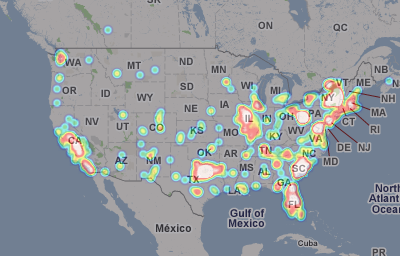
\includegraphics[bb=0 0 400 256]{img/cs-classic.png}
\caption{classic}\label{fig:classic}
\end{figure}

\begin{figure}[htp]

\includegraphics[bb=0 0 24 256]{color-schemes/fire.png}
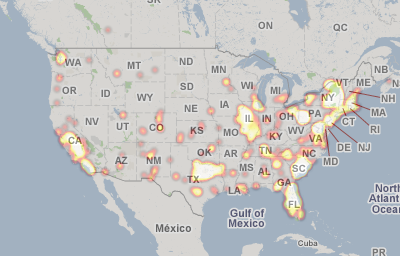
\includegraphics[bb=0 0 400 256]{img/cs-fire.png}
\caption{fire}\label{fig:fire}
\end{figure}

\begin{figure}[htp]

\includegraphics[bb=0 0 24 256]{color-schemes/omg.png}
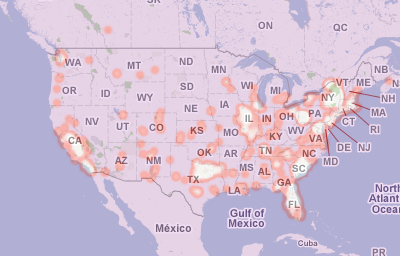
\includegraphics[bb=0 0 400 256]{img/cs-omg.png}
\caption{omg}\label{fig:omg}
\end{figure}

\begin{figure}[htp]

\includegraphics[bb=0 0 24 256]{color-schemes/pgaitch.png}
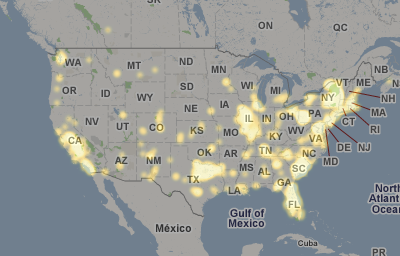
\includegraphics[bb=0 0 400 256]{img/cs-pgaitch.png}
\caption{pgaitch}\label{fig:pgaitch}
\end{figure}

\begin{figure}[htp]

\includegraphics[bb=0 0 24 256]{color-schemes/pbj.png}
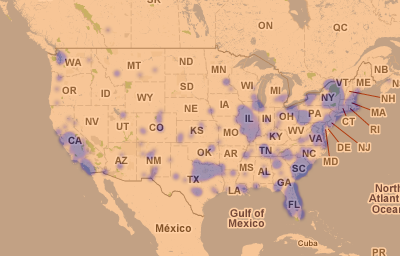
\includegraphics[bb=0 0 400 256]{img/cs-pbj.png}
\caption{pbj}\label{fig:pbj}
\end{figure}

You can produce your own color scheme. A color scheme is defined by a PNG of
height 256 pixels. The image may be as wide as you like; only the first column
of pixels will be looked at. This first column is effectively a mapping of
intensities to four-channel colors (red, green, blue, and alpha). To use a
custom color scheme, place your PNG file in the \file{__/etc/color-schemes/}
directory of your Gheat installation, and use your PNG's filename without the
\file{.png} extension as the token to wire into your JavaScript.

The alpha channel of the pixels in the color scheme are multiplied with the
master opacity setting for the given zoom level (see above) to determine the 
final opacity of a given pixel in each tile.

If and when you change the PNG file for a color scheme of a given name, you
need to manually delete the tile cache for that color scheme.

\begin{seealso}

\seelink{http://www.zetadev.com/software/aspen/0.8/doc/html/aspen-conf.html}{\file{aspen.conf}}{Documentation for the \file{aspen.conf} file}

\seelink{http://docs.python.org/lib/module-ConfigParser.html}{\module{ConfigParser}}{This
describes the \file{INI} format used in \file{aspen.conf} (the
\class{RawConfigParser} is used)}

\end{seealso}


\chapter{The db.py script}
\label{db.py}

The script at \file{__/bin/db.py} is used to manage the database at 
\file{__/var/points.db}. It's available subcommands are:

\begin{tableii}{l|l}{var}{Subcommand}{Description}
\lineii{clear}{Remove all points from the database}
\lineii{count}{Print the number of points in the database to \file{stdout}}
\lineii{delete}{Delete the database from the filesystem}
\lineii{sync}{Update the database from the file at \file{__/var/points.txt}}
\end{tableii}

For the \var{clear}, \var{count}, and \var{sync} subcommands, the database will
be created if it does not exist. The default subcommand is \var{sync}. 

The \file{__/var/points.txt} file is a CSV-formatted file with three fields:
\var{point id}, \var{latitude}, and \var{longitude}. The \var{point id} field
can be any string. If it is not unique within the \file{points.txt} file then
the last point with a given \var{point id} will override any previous points
with that same \var{point id}. Gheat uses the \var{point id} field to keep
track of when points should be removed from the database, as well as when
points are updated, in order to tell when the tile cache ought to be flushed.
The \var{latitude} and \var{longitude} fields must be floats. Multiple data
points may have the same latitude and longitude in order to increase the
intensity of that geographic point on the heatmap.

The \var{sync} subcommand outputs a token for each point in the
\file{points.txt} file:

\begin{tableii}{l|l}{code}{Token}{Meaning}
\lineii{.}{The point was not modified since the last time it was seen}
\lineii{o}{The point was modified and has been updated}
\lineii{O}{This is a new point}
\end{tableii}

The number of points deleted can be determined by using the \var{count}
subcommand before and after the \var{sync} subcommand.


\end{document}
